\only<1-2>{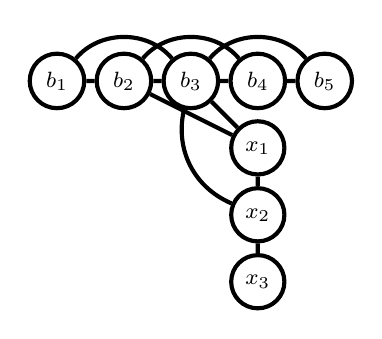
\begin{tikzpicture}[scale=0.85]

    \node[circle, draw=black, fill=white, line width=1.5pt, font=\footnotesize] (b2) at (0, 2) {$b_1$};
    \node[circle, draw=black, fill=white, line width=1.5pt, font=\footnotesize] (b1) at (1, 2) {$b_2$};
    \node[circle, draw=black, fill=white, line width=1.5pt, font=\footnotesize] (b0) at (2, 2) {$b_3$};
    
    \node[circle, draw=black, fill=white, line width=1.5pt, font=\footnotesize] (x5) at (3, -1) {$x_{3}$};
    \node[circle, draw=black, fill=white, line width=1.5pt, font=\footnotesize] (x6) at (3, 0) {$x_{2}$};
    \node[circle, draw=black, fill=white, line width=1.5pt, font=\footnotesize] (x7) at (3, 1) {$x_{1}$};
    

    \draw[line width=1.5pt] (b0) to (b1);
    \draw[line width=1.5pt] (b1) to (b2);
    \draw[line width=1.5pt, bend right=50] (b0) to (b2);


    \draw[line width=1.5pt] (x5) to (x6);
    \draw[line width=1.5pt] (x6) to (x7);

    \draw[line width=1.5pt] (b0) to (x7);
    \draw[line width=1.5pt, bend right=40] (b0) to (x6);
    \draw[line width=1.5pt] (b1) to (x7);
    
    \onslide<2>{
        \node[circle, draw=black, fill=white, line width=1.5pt, font=\footnotesize] (b3) at (3, 2) {$b_4$};
        \node[circle, draw=black, fill=white, line width=1.5pt, font=\footnotesize] (b4) at (4, 2) {$b_5$};
        \draw[line width=1.5pt] (b0) to (b3);
        \draw[line width=1.5pt] (b3) to (b4);
        \draw[line width=1.5pt, bend left=50] (b1) to (b3);
        \draw[line width=1.5pt, bend left=50] (b0) to (b4);
    }
\end{tikzpicture}
}
\only<3>{\begin{tikzpicture}[scale=0.85]

    \node[circle, draw=black, fill=white, line width=1.5pt, font=\footnotesize] (b2) at (0, 2) {$b_1$};
    \node[circle, draw=black, fill=white, line width=1.5pt, font=\footnotesize] (b1) at (1, 2) {$b_2$};
    \node[circle, draw=black, fill=cfred, line width=1.5pt, font=\footnotesize] (b0) at (2, 2) {$b_3$};
    
    \node[circle, draw=black, fill=white, line width=1.5pt, font=\footnotesize] (x5) at (3, -1) {$x_{3}$};
    \node[circle, draw=black, fill=white, line width=1.5pt, font=\footnotesize] (x6) at (3, 0) {$x_{2}$};
    \node[circle, draw=black, fill=white, line width=1.5pt, font=\footnotesize] (x7) at (3, 1) {$x_{1}$};
    

    \draw[line width=1.5pt] (b0) to (b1);
    \draw[line width=1.5pt] (b1) to (b2);
    \draw[line width=1.5pt, bend right=50] (b0) to (b2);


    \draw[line width=1.5pt] (x5) to (x6);
    \draw[line width=1.5pt] (x6) to (x7);

    \draw[line width=1.5pt] (b0) to (x7);
    \draw[line width=1.5pt, bend right=40] (b0) to (x6);
    \draw[line width=1.5pt] (b1) to (x7);
    
        \node[circle, draw=black, fill=cfred, line width=1.5pt, font=\footnotesize] (b3) at (3, 2) {$b_4$};
        \node[circle, draw=black, fill=cfred, line width=1.5pt, font=\footnotesize] (b4) at (4, 2) {$b_5$};
        \draw[line width=1.5pt] (b0) to (b3);
        \draw[line width=1.5pt] (b3) to (b4);
        \draw[line width=1.5pt, bend left=50] (b1) to (b3);
        \draw[line width=1.5pt, bend left=50] (b0) to (b4);
\end{tikzpicture}
}
\only<4>{\begin{tikzpicture}[scale=0.85]

    \node[circle, draw=black, fill=white, line width=1.5pt, font=\footnotesize] (b2) at (0, 2) {$b_1$};
    \node[circle, draw=black, fill=cfred, line width=1.5pt, font=\footnotesize] (b1) at (1, 2) {$b_2$};
    \node[circle, draw=black, fill=cfred, line width=1.5pt, font=\footnotesize] (b0) at (2, 2) {$b_3$};
    
    \node[circle, draw=black, fill=white, line width=1.5pt, font=\footnotesize] (x5) at (3, -1) {$x_{3}$};
    \node[circle, draw=black, fill=white, line width=1.5pt, font=\footnotesize] (x6) at (3, 0) {$x_{2}$};
    \node[circle, draw=black, fill=white, line width=1.5pt, font=\footnotesize] (x7) at (3, 1) {$x_{1}$};
    

    \draw[line width=1.5pt] (b0) to (b1);
    \draw[line width=1.5pt] (b1) to (b2);
    \draw[line width=1.5pt, bend right=50] (b0) to (b2);


    \draw[line width=1.5pt] (x5) to (x6);
    \draw[line width=1.5pt] (x6) to (x7);

    \draw[line width=1.5pt] (b0) to (x7);
    \draw[line width=1.5pt, bend right=40] (b0) to (x6);
    \draw[line width=1.5pt] (b1) to (x7);
    
        \node[circle, draw=black, fill=cfred, line width=1.5pt, font=\footnotesize] (b3) at (3, 2) {$b_4$};
        \node[circle, draw=black, fill=cfred!20, line width=1.5pt, font=\footnotesize] (b4) at (4, 2) {$b_5$};
        \draw[line width=1.5pt] (b0) to (b3);
        \draw[line width=1.5pt] (b3) to (b4);
        \draw[line width=1.5pt, bend left=50] (b1) to (b3);
        \draw[line width=1.5pt, bend left=50] (b0) to (b4);
\end{tikzpicture}
}
\only<5>{\begin{tikzpicture}[scale=0.85]

    \node[circle, draw=black, fill=white, line width=1.5pt, font=\footnotesize] (b2) at (0, 2) {$b_1$};
    \node[circle, draw=black, fill=cfred, line width=1.5pt, font=\footnotesize] (b1) at (1, 2) {$b_2$};
    \node[circle, draw=black, fill=cfred, line width=1.5pt, font=\footnotesize] (b0) at (2, 2) {$b_3$};
    
    \node[circle, draw=black, fill=white, line width=1.5pt, font=\footnotesize] (x5) at (3, -1) {$x_{3}$};
    \node[circle, draw=black, fill=white, line width=1.5pt, font=\footnotesize] (x6) at (3, 0) {$x_{2}$};
    \node[circle, draw=black, fill=cfred, line width=1.5pt, font=\footnotesize] (x7) at (3, 1) {$x_{1}$};
    

    \draw[line width=1.5pt] (b0) to (b1);
    \draw[line width=1.5pt] (b1) to (b2);
    \draw[line width=1.5pt, bend right=50] (b0) to (b2);


    \draw[line width=1.5pt] (x5) to (x6);
    \draw[line width=1.5pt] (x6) to (x7);

    \draw[line width=1.5pt] (b0) to (x7);
    \draw[line width=1.5pt, bend right=40] (b0) to (x6);
    \draw[line width=1.5pt] (b1) to (x7);
    
        \node[circle, draw=black, fill=cfred!20, line width=1.5pt, font=\footnotesize] (b3) at (3, 2) {$b_4$};
        \node[circle, draw=black, fill=white, line width=1.5pt, font=\footnotesize] (b4) at (4, 2) {$b_5$};
        \draw[line width=1.5pt] (b0) to (b3);
        \draw[line width=1.5pt] (b3) to (b4);
        \draw[line width=1.5pt, bend left=50] (b1) to (b3);
        \draw[line width=1.5pt, bend left=50] (b0) to (b4);
\end{tikzpicture}
}
\only<6>{\begin{tikzpicture}[scale=0.85]

    \node[circle, draw=black, fill=white, line width=1.5pt, font=\footnotesize] (b2) at (0, 2) {$b_1$};
    \node[circle, draw=black, fill=cfred!20, line width=1.5pt, font=\footnotesize] (b1) at (1, 2) {$b_2$};
    \node[circle, draw=black, fill=cfred, line width=1.5pt, font=\footnotesize] (b0) at (2, 2) {$b_3$};
    
    \node[circle, draw=black, fill=white, line width=1.5pt, font=\footnotesize] (x5) at (3, -1) {$x_{3}$};
    \node[circle, draw=black, fill=cfred, line width=1.5pt, font=\footnotesize] (x6) at (3, 0) {$x_{2}$};
    \node[circle, draw=black, fill=cfred, line width=1.5pt, font=\footnotesize] (x7) at (3, 1) {$x_{1}$};
    

    \draw[line width=1.5pt] (b0) to (b1);
    \draw[line width=1.5pt] (b1) to (b2);
    \draw[line width=1.5pt, bend right=50] (b0) to (b2);


    \draw[line width=1.5pt] (x5) to (x6);
    \draw[line width=1.5pt] (x6) to (x7);

    \draw[line width=1.5pt] (b0) to (x7);
    \draw[line width=1.5pt, bend right=40] (b0) to (x6);
    \draw[line width=1.5pt] (b1) to (x7);
    
        \node[circle, draw=black, fill=white, line width=1.5pt, font=\footnotesize] (b3) at (3, 2) {$b_4$};
        \node[circle, draw=black, fill=white, line width=1.5pt, font=\footnotesize] (b4) at (4, 2) {$b_5$};
        \draw[line width=1.5pt] (b0) to (b3);
        \draw[line width=1.5pt] (b3) to (b4);
        \draw[line width=1.5pt, bend left=50] (b1) to (b3);
        \draw[line width=1.5pt, bend left=50] (b0) to (b4);
\end{tikzpicture}
}
\only<7>{\begin{tikzpicture}[scale=0.85]

    \node[circle, draw=black, fill=white, line width=1.5pt, font=\footnotesize] (b2) at (0, 2) {$b_1$};
    \node[circle, draw=black, fill=white, line width=1.5pt, font=\footnotesize] (b1) at (1, 2) {$b_2$};
    \node[circle, draw=black, fill=cfred!20, line width=1.5pt, font=\footnotesize] (b0) at (2, 2) {$b_3$};
    
    \node[circle, draw=black, fill=cfred, line width=1.5pt, font=\footnotesize] (x5) at (3, -1) {$x_{3}$};
    \node[circle, draw=black, fill=cfred, line width=1.5pt, font=\footnotesize] (x6) at (3, 0) {$x_{2}$};
    \node[circle, draw=black, fill=cfred, line width=1.5pt, font=\footnotesize] (x7) at (3, 1) {$x_{1}$};
    

    \draw[line width=1.5pt] (b0) to (b1);
    \draw[line width=1.5pt] (b1) to (b2);
    \draw[line width=1.5pt, bend right=50] (b0) to (b2);


    \draw[line width=1.5pt] (x5) to (x6);
    \draw[line width=1.5pt] (x6) to (x7);

    \draw[line width=1.5pt] (b0) to (x7);
    \draw[line width=1.5pt, bend right=40] (b0) to (x6);
    \draw[line width=1.5pt] (b1) to (x7);
    
        \node[circle, draw=black, fill=white, line width=1.5pt, font=\footnotesize] (b3) at (3, 2) {$b_4$};
        \node[circle, draw=black, fill=white, line width=1.5pt, font=\footnotesize] (b4) at (4, 2) {$b_5$};
        \draw[line width=1.5pt] (b0) to (b3);
        \draw[line width=1.5pt] (b3) to (b4);
        \draw[line width=1.5pt, bend left=50] (b1) to (b3);
        \draw[line width=1.5pt, bend left=50] (b0) to (b4);
\end{tikzpicture}
}